\documentclass[../notes.tex]{subfiles}

\pagestyle{main}
\renewcommand{\chaptermark}[1]{\markboth{\chaptername\ \thechapter\ (#1)}{}}
\stepcounter{chapter}

\begin{document}




\chapter{Cycloadditions and Photochemistry}
\section{Problems 2 and 5}
\begin{itemize}
    \item \marginnote{9/6:}We begin with Problem 5.
    \begin{figure}[h!]
        \centering
        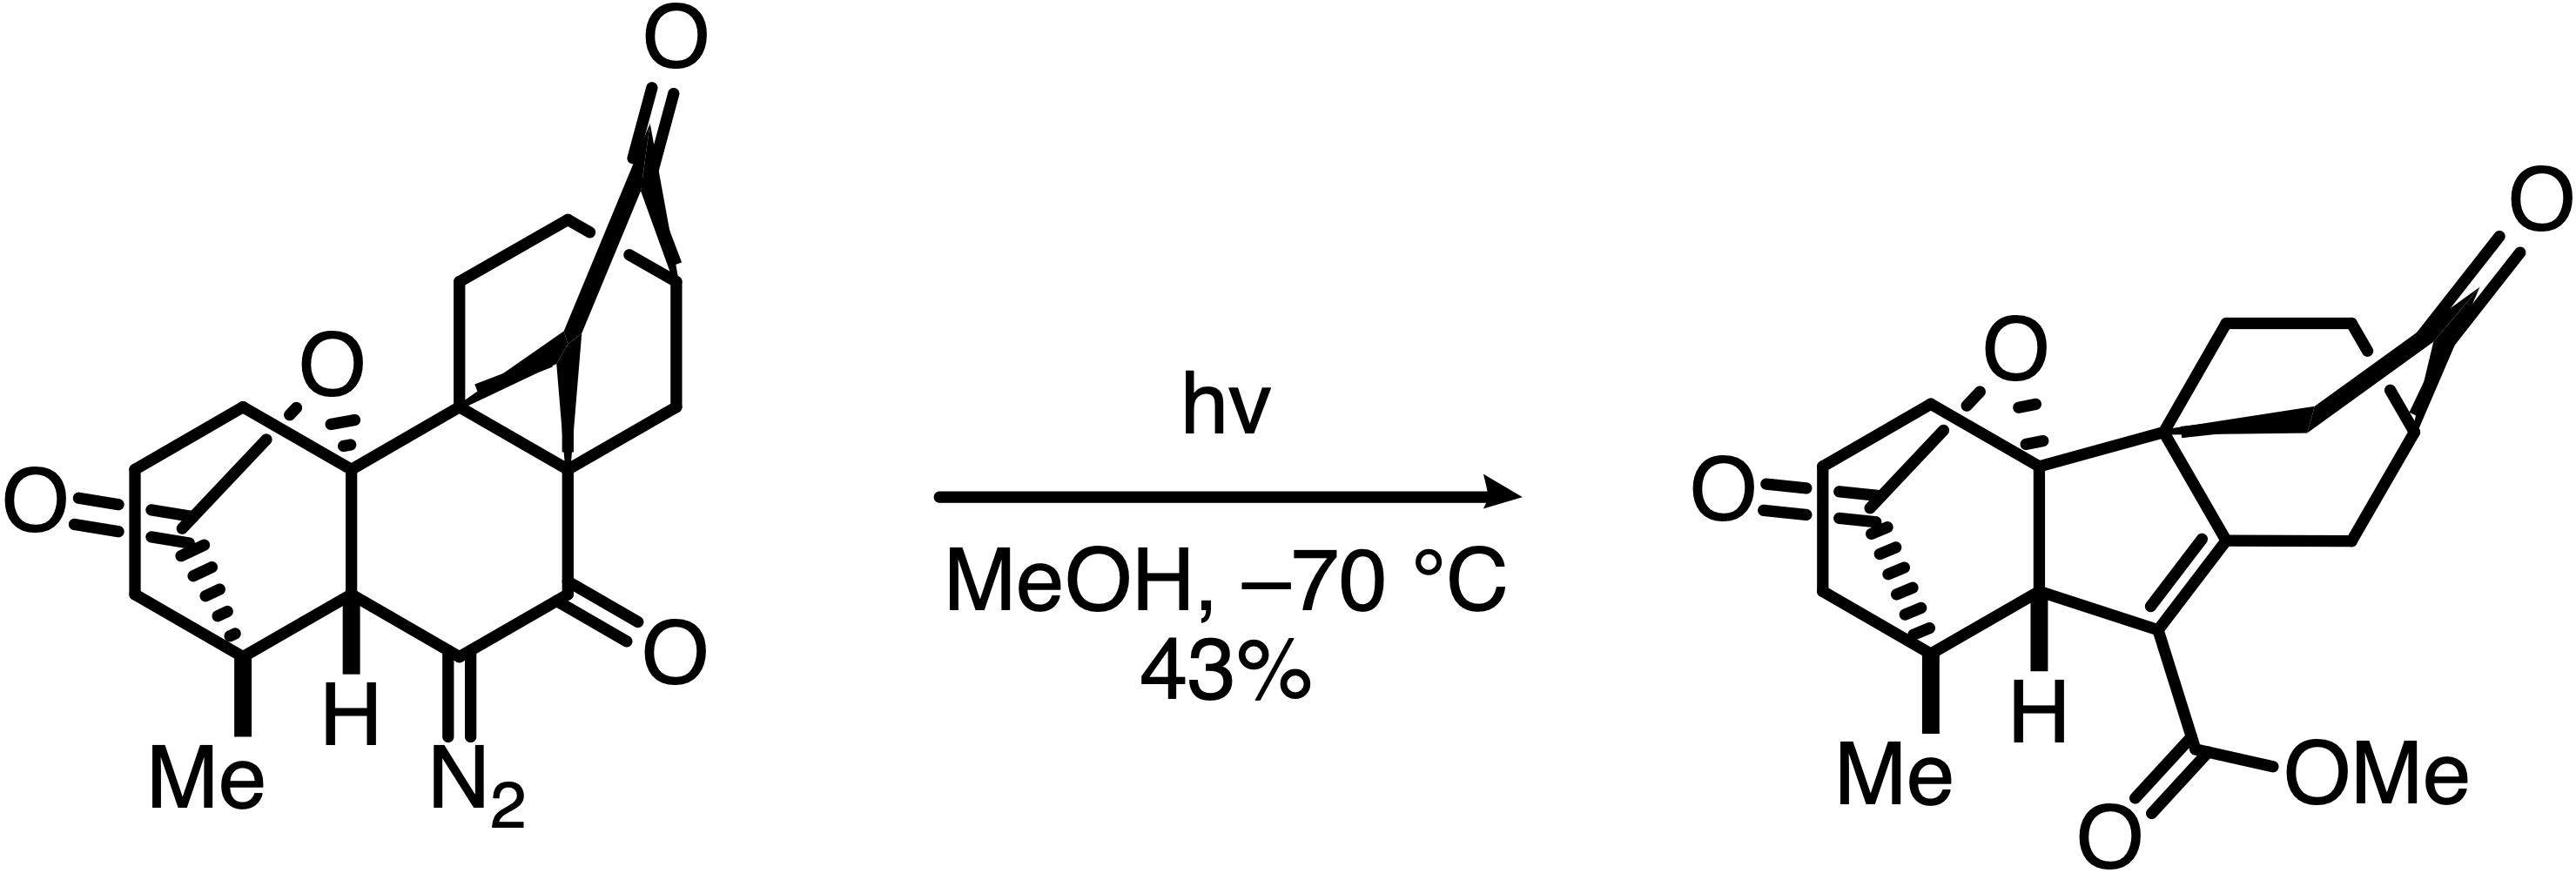
\includegraphics[width=0.5\linewidth]{PSet2Q5.png}
        \caption{PSet 2, Q5.}
        \label{fig:PSet2Q5}
    \end{figure}
    \item The first step --- and the light-activated step --- is a photolytic \textbf{Wolff rearrangement}.
    \begin{itemize}
        \item Specifically, the light will photoexcite the diazo functional group. We don't really need to show this, though.
    \end{itemize}
    \item After that, we have methanol addition to the ketene.
    \begin{itemize}
        \item By using two methanol molecules, we can access a six-membered transition state.
        \item On ketenes.
        \begin{itemize}
            \item The \ce{C=O} and \ce{C=C} $\pi$-bonding orbitals are orthogonal.
            \item More specifically, this means that the \ce{C=O} $\pi$-bond orbital lies in the plane of the page, and the \ce{C=C} $\pi$-bond orbital lies out of the plane of the page.
        \end{itemize}
        \item Implication: We must be careful about choosing the side of the ketene to which the methanol adds.
    \end{itemize}
    \item Hydrogen bonding from methanol stabilizes many of the steps, as drawn in the third intermediate.
    \item There may be a \textbf{retro-Michael addition} somewhere in here. However, this was said to form an enolate, and thus be a step we'd like to avoid??
    \item Jasmin: Where can we learn about photoexcitation problems?
    \begin{itemize}
        \item There are two types of photoexcitation regimes: Broad spectrum and specific wavelength.
        \item The majority of productive photochemical processes use lower energy photons.
        \begin{itemize}
            \item As a consequence, photochemistry is rare among unsaturated systems because anything powerful enough to drive something there will rupture bonds everywhere.
        \end{itemize}
        \item By contrast, conjugated systems are more easily photoexcited.
        \item Example: The most reliable way to generate 4-membered rings is with photoexcitation! We can form 4-membered rings in such a system because we're pumping more than enough energy to overcome the ring strain. Here's how it works.
        \begin{figure}[h!]
            \centering
            \footnotesize
            \schemestart
                \chemfig{-[:30](=[2]O)-[:-30]=_[6]}
                \arrow{->[$h\nu$]}
                \chemleft[
                    \subscheme{
                        \chemfig{-[:30](-[2]\charge{30=\.}{O})=_[:-30]-[6]\charge{0=\.}{}}
                        \arrow{<->}
                        \chemfig{-[:30](=[2]O)-[:-30]\charge{0=\.}{}-[6]\charge{0=\.}{}-[,0.3,,,opacity=0]}
                    }
                \chemright]
                \arrow{->[\chemfig[atom sep=1em]{*6(-----=)}]}
                \chemfig{-[:30](=[2]O)-[:-30]\charge{30=\.}{}-[6]-*6([:30]-----\charge{150=\.}{}-)}
                \arrow
                \chemfig{-[:30](=[2]O)-[:-30]*4([:-45]--*6(-----)--)}
            \schemestop
            \caption{Forming 4-membered rings via photochemistry.}
            \label{fig:4photo}
        \end{figure}
        \begin{itemize}
            \item A $\beta$-unsaturated carbonyl can be excited to a diradical, which can also be thought of as an exited state of the $\pi$-bond.
            \begin{itemize}
                \item Note that the unconjugated alkene does \emph{not} get photoexcited!
            \end{itemize}
            \item Then we can do radical chemistry with the ketone, which is hard to excite.
        \end{itemize}
        \item You could also have photoexcitation followed by intersystem crossing (singlet to triplet state).
        \item We will likely learn more about photoexcitation in 5.53.
        \item Takeaway: Looking at the starting material, we should identify conjugated systems, like how the ketone is conjugated to the $\beta$-\ce{C=N} bond.
    \end{itemize}
    \item Aside: Rhodium can do very similar chemistry under thermal conditions. Instead of a carbene, we'd get a metal alkylidene, but it'd be the same end product.
    \begin{itemize}
        \item So this can be transition-metal catalyzed.
    \end{itemize}
    \item Reference: \textcite{bib:PSet2Q5}.
    \item Altogether, the full solution to PSet 2, Q5 is on the next page.
    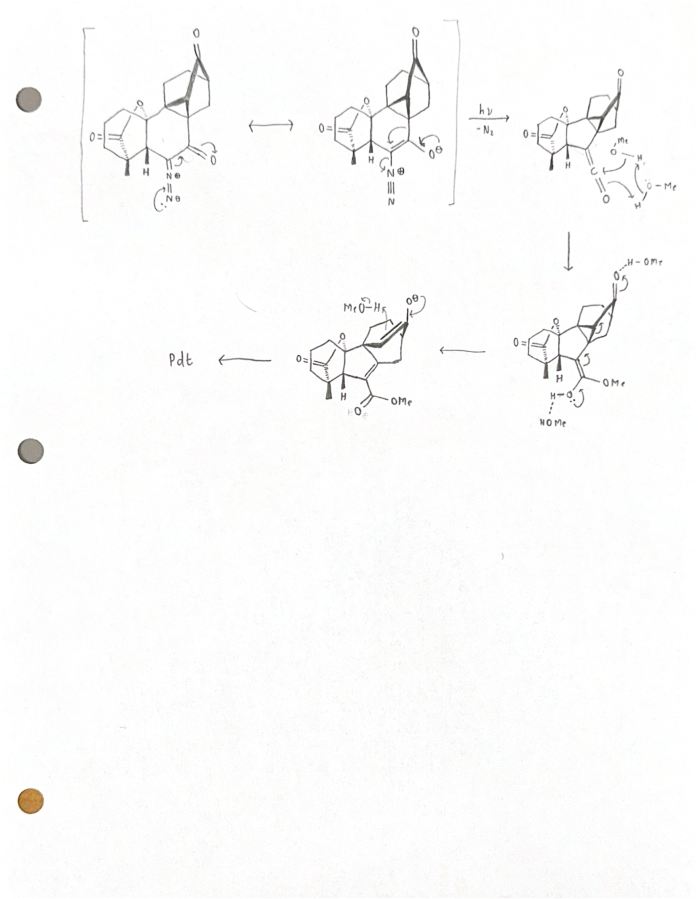
\includepdf{ExtFiles/PSet2Q5Full.pdf}
    \item We now begin Problem 2.
    \begin{figure}[h!]
        \centering
        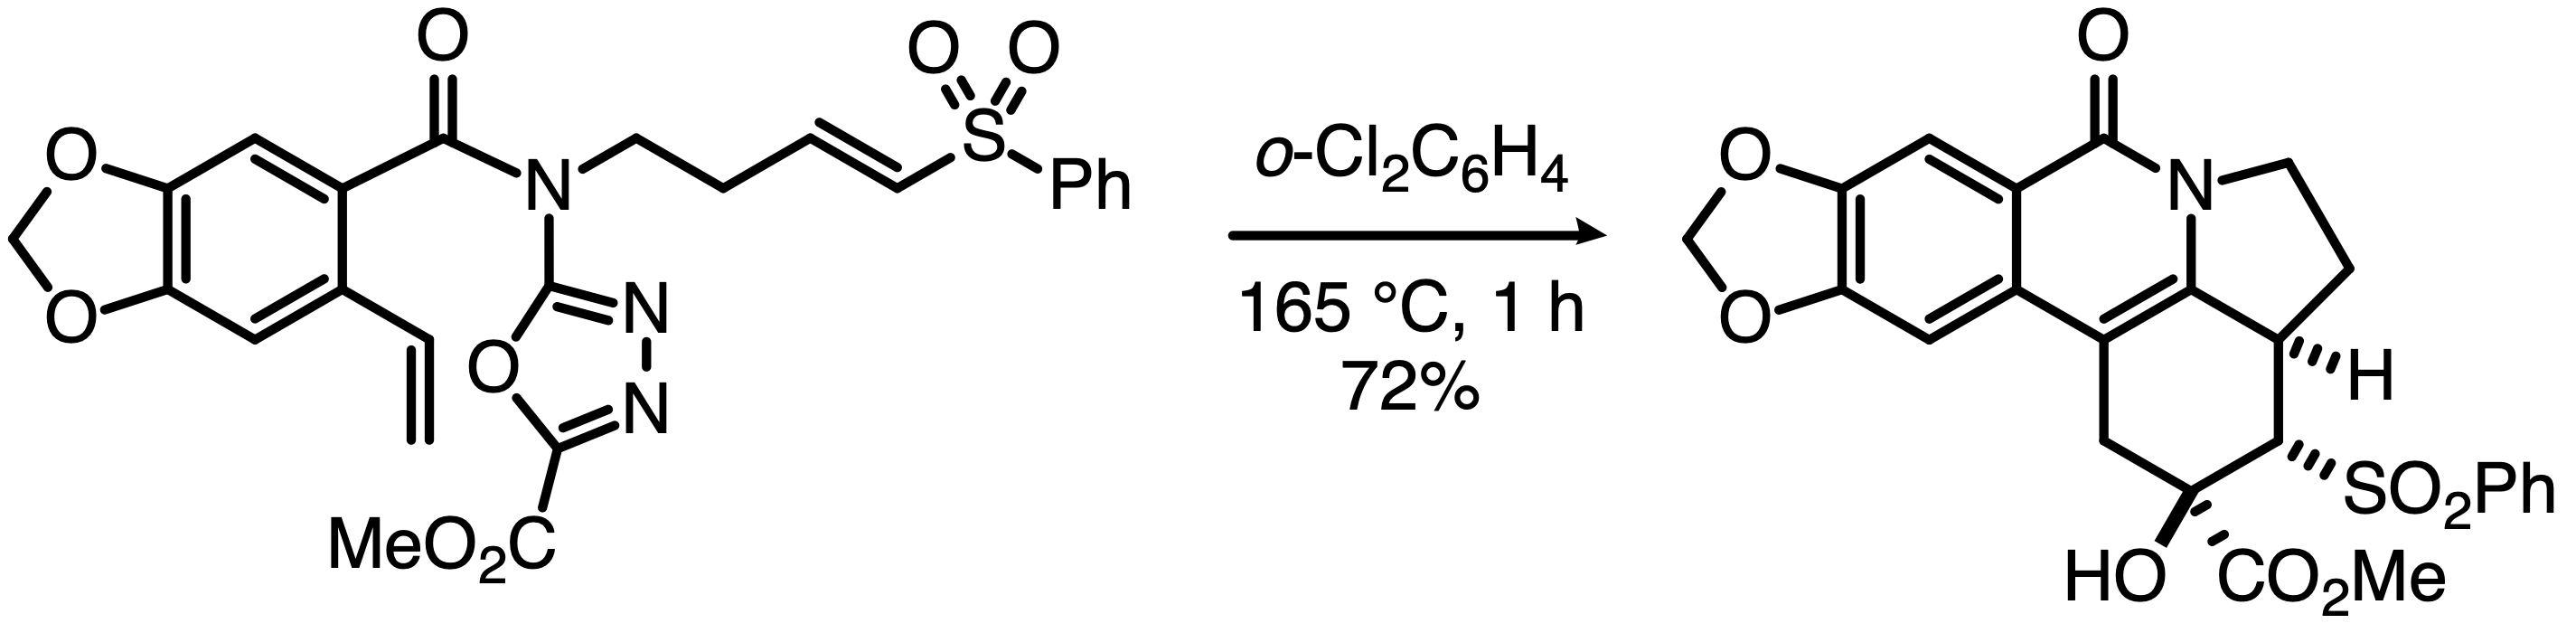
\includegraphics[width=0.65\linewidth]{PSet2Q2.png}
        \caption{PSet 2, Q2.}
        \label{fig:PSet2Q2}
    \end{figure}
    \item Starts off with a $[4+2]$ cycloaddition, which will follow similar rules to the analogous Diels-Alder.
    \begin{itemize}
        \item For example, this cycloaddition will also be diastereoselective, and hence will prefer to have the phenylsulfonyl EWG be \emph{endo} in the transition state.
        \begin{itemize}
            \item This sets the stereochemistry of the right side of the molecule.
        \end{itemize}
        \item This is an antarafacial/suprafacial reaction, not a suprafacial/suprafacial reaction.
        \begin{itemize}
            \item Read up on the \textbf{Woodward-Hoffmann rules}!!
        \end{itemize}
        \item Forming a 5-membered ring is better than a six-membered ring??
        \item Note that we choose to react with the more electron-poor alkene because it has a lower, more energetically accessible LUMO.
    \end{itemize}
    \item After the cycloaddition, we rearrange the electrons and spit out nitrogen.
    \item We then do another $[4+2]$ cycloaddition.
    \begin{itemize}
        \item How do we retain the stereochemistry at the carbanion?? What's the alternate mechanism?
    \end{itemize}
    \item At high temperature, the \ce{N-O} ketal can drop down and (reversibly) expel the oxygen.
    \begin{itemize}
        \item The formation of the \ce{N}-acyl iminium will seriously labilize the $\alpha$-carbon's hydrogens. The labilization effect is so extreme that any base in solution --- from the starting material, to something intramolecular, to the unsilylated glass of the reaction vessel --- will pick it off.
    \end{itemize}
    \item Then we just have to protonate the oxygen and we're done!
    \item Altogether, the full solution to PSet 2, Q2 is on the next page.
    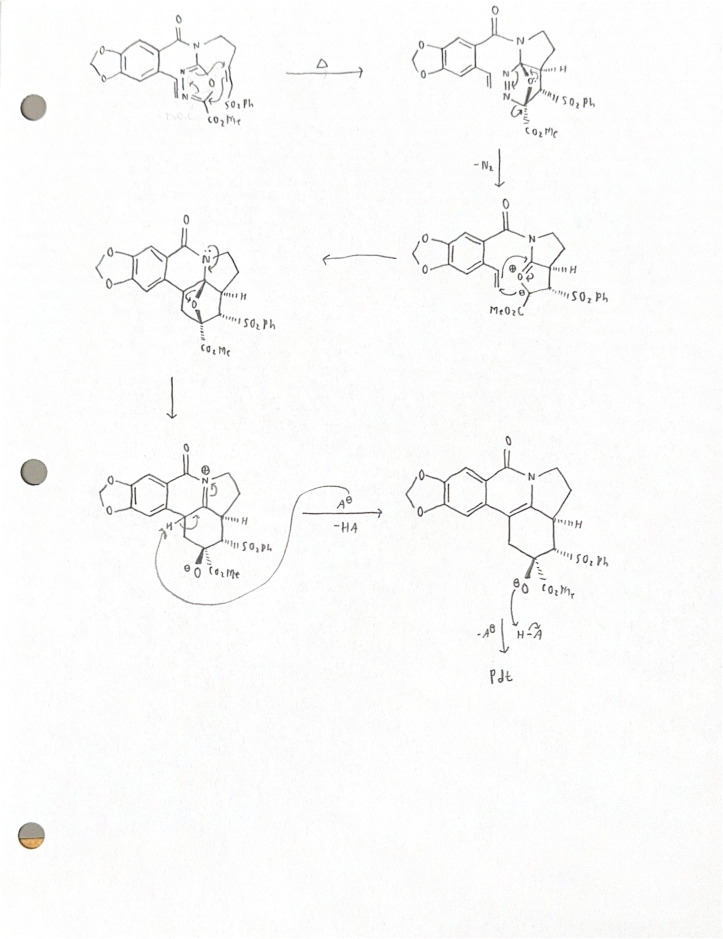
\includepdf{ExtFiles/PSet2Q2Full.pdf}
    \item Definitely have all of PSet 2 ready for next Monday!! And have at least looked at PSet 3.
    \begin{itemize}
        \item PSet 2, Q3 is gonna need really good 3D transition state structures. Make sure to try this one!! Hints:
        \begin{itemize}
            \item You start with a Diels-Alder. Lewis acid activates the ketone.
            \item This lowers the energy of the LUMO; sets the stage for an intramolecular Diels-Alder.
            \item Following this, draw the intermediate, put it in a chair scenario, and then sort out the azide.
            \item Azides and Lewis acids can add into the carbonyl. This will lead to loss of \ce{N2}, and how can we facilitate this?
            \begin{itemize}
                \item Schmidt reaction.
            \end{itemize}
            \item Lots of antiperiplanar interactions that are responsible for product distribution.
            \begin{itemize}
                \item This problem is something of a sequel to PSet 1, Q3.
            \end{itemize}
        \end{itemize}
        \item We will start next time with PSet 2, Q3.
    \end{itemize}
    \item Remember to take more pictures!!
    \item Use whatever time we have for this class to think about future problems, not clean copying notes.
    \item Jasmin and I will start next time with two PSet 2 problems; one of us will take Q3, the other Q1.
    \item Focus on PSet 2, but we can start PSet 3.
\end{itemize}



\section{Problems 1, 3, 4, and 6}
\begin{itemize}
    \item \marginnote{9/9:}What is the up/down arrow symbol in Problem 4?
    \begin{itemize}
        \item Means reflux (e.g., heat).
    \end{itemize}
    \item We now begin discussing Problem 3.
    \begin{figure}[h!]
        \centering
        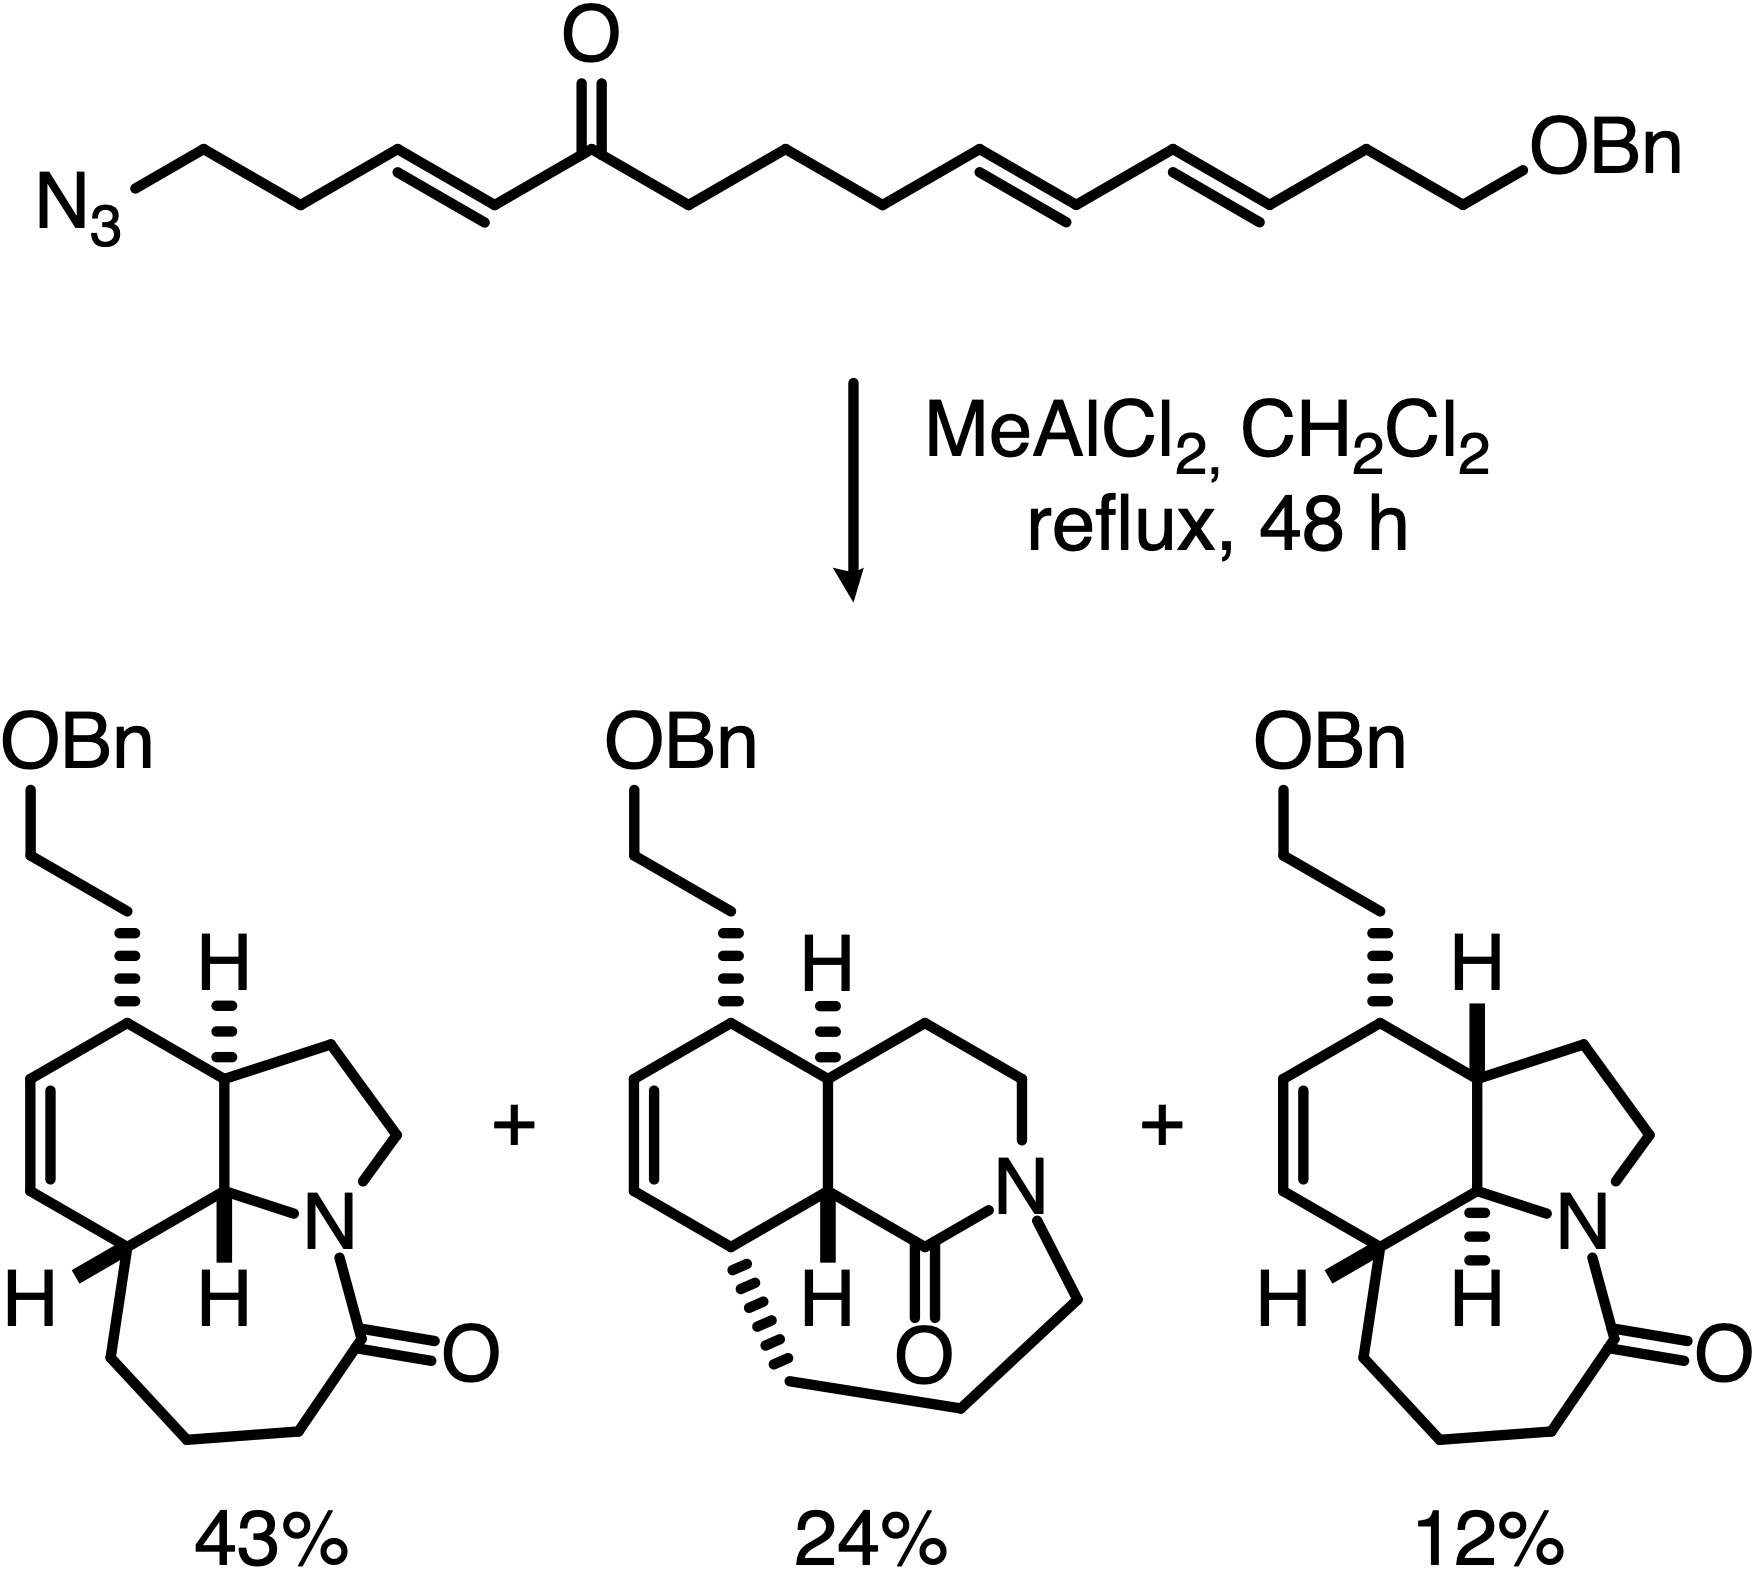
\includegraphics[width=0.4\linewidth]{PSet2Q3.png}
        \caption{PSet 2, Q3.}
        \label{fig:PSet2Q3}
    \end{figure}
    \item \ce{MeAlCl2} is a common Lewis acid catalyst for Diels-Alder reactions. As such, we will begin with coordination of the ketone EWG on the dienophile to \ce{MeAlCl2} to further activate it.
    \begin{itemize}
        \item This activated EWG will lower the LUMO of the dieneophile.
    \end{itemize}
    \item Even after this activation step, however, we will still need reflux conditions for this Diels-Alder to proceed because the diene is only activated inductively through hyperconjugation.
    \item Also note that to lead into the Diels-Alder, we may need to redraw the substrate in the more favorable s-\emph{cis} conformation.
    \begin{itemize}
        \item We also bring the diene closer to the dienophile spatially.
        \item Numbering the carbons can help with drawing this change.
    \end{itemize}
    \item It is important to note that there are two possible Diels-Alder conformations: \emph{exo} and \emph{endo}.
    \begin{itemize}
        \item The transition state with the ketone (the EWG) on the outside is the \emph{exo} TS.
        \item The transition state with the ketone over the diene is the \emph{endo} TS.
        \item \emph{endo} is favored by electronics and will lead to the two major products.
        \item \emph{endo} transition state is preferred for intermolecular, but for intramolecular, we may see more of the \emph{exo} transition state!
        \item Let's look at the \emph{exo} pathway first since it only leads to one product.
    \end{itemize}
    \item We now proceed with the Diels-Alder.
    \begin{itemize}
        \item Because the Diels-Alder is famously diastereoselective, the product's stereochemistry is set here.
        \begin{itemize}
            \item More specifically, the Diels-Alder is \textbf{stereospecific}, not \textbf{stereoselective}.
            \item Also notice that we have 3 \emph{E} alkenes in the starting material.
        \end{itemize}
        \item We will, however, obtain $(+/-)$-products, depending on whether the diene attacks the dienophile from the top face or bottom face.
        \item To yield the entaniomer shown, we need the diene to attack the dienophile from the top.
    \end{itemize}
    \item \textbf{Stereospecific} (reaction): A chemical reaction that yields a single stereoisomer as the sole product.
    \item \textbf{Stereoselective} (reaction): A chemical reaction that favors one stereoisomer over others but can still produce a mixture of stereoisomers.
    \item We should recognize that the Diels-Alder forms the equivalent of a substituted decalin.
    \begin{itemize}
        \item Thus, we can choose between \emph{cis}-decalin and \emph{trans}-decalin for our chair conformation.
        \begin{itemize}
            \item When we draw decalins, it is good to draw the stereodetermining hydrides, too.
        \end{itemize}
        \item This is a bit of a stretch as the alkene will enforce a flat \emph{cis} conformation where it is, but we can just modify the chair structure.
        \item It is also good to work out the stereochemistry in 2D first, and then translate it to 3D.
        \item Pay attention to chair conformations, too: You want to make sure that your substituents are arranged in the more energetically favorable conformation and not clashing.
    \end{itemize}
    \item Immediately after the Diels-Alder, we begin an intramolecular Schmidt reaction.
    \begin{itemize}
        \item The negative charge at the end of the azide helps push the near double bond electrons toward the activated carbonyl.
    \end{itemize}
    \item After this first step, the rest of the azide can be either axial or equatorial on the 6-membered heterocycle, and we'll likely have rapid epimerization because stereochemistry is not fixed at nitrogen atoms.
    \item When the rest of the azide is equatorial, it is antiperiplanar to one of the \ce{C-C} bonds adjacent to the oxygen.
    \begin{itemize}
        \item In this conformation, that bond can disengage to attack the $\sigma^*$-orbital of the \ce{N-N} single bond.
    \end{itemize}
    \item This final step yields the most minor product.
    \item The other two products will come from the \emph{endo}-pathway. We will get two products in the other pathway because the azide epimerization puts \emph{two} \ce{C-C} bonds antiperiplanar to the \ce{N-N} single bond.
    \item Altogether, the full \emph{exo} pathway for PSet 2, Q3 is on the next page.
    \begin{itemize}
        \item Note that the rewrite to the 3D form and the rewrite back both accidentally involve shifts to the other enantiomer.
    \end{itemize}
    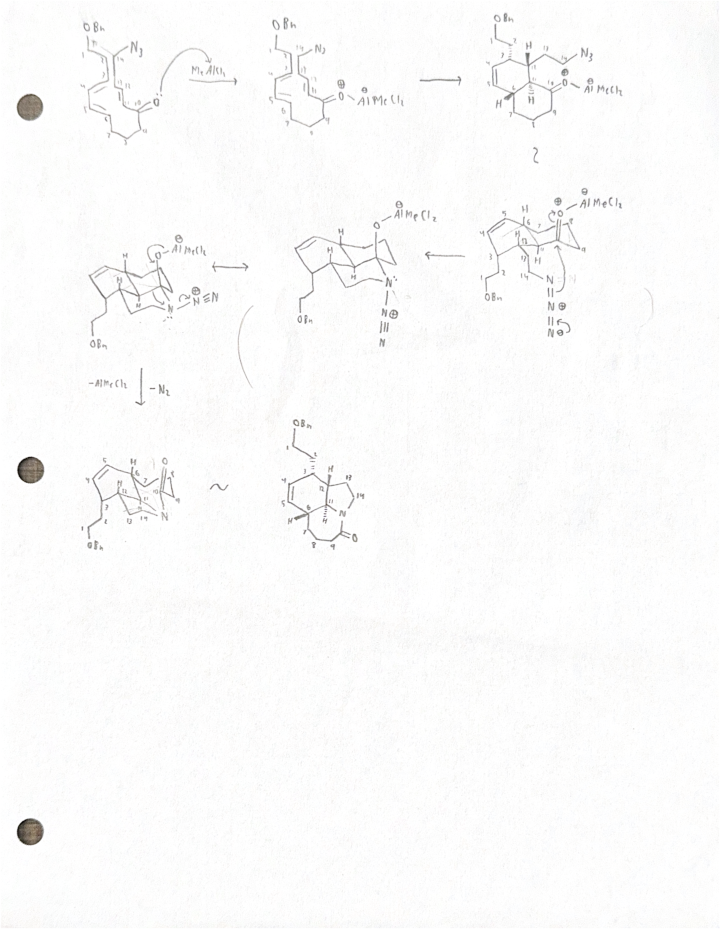
\includepdf{ExtFiles/PSet2Q3Exo.pdf}
    \item We now begin discussing Problem 1.
    \begin{figure}[h!]
        \centering
        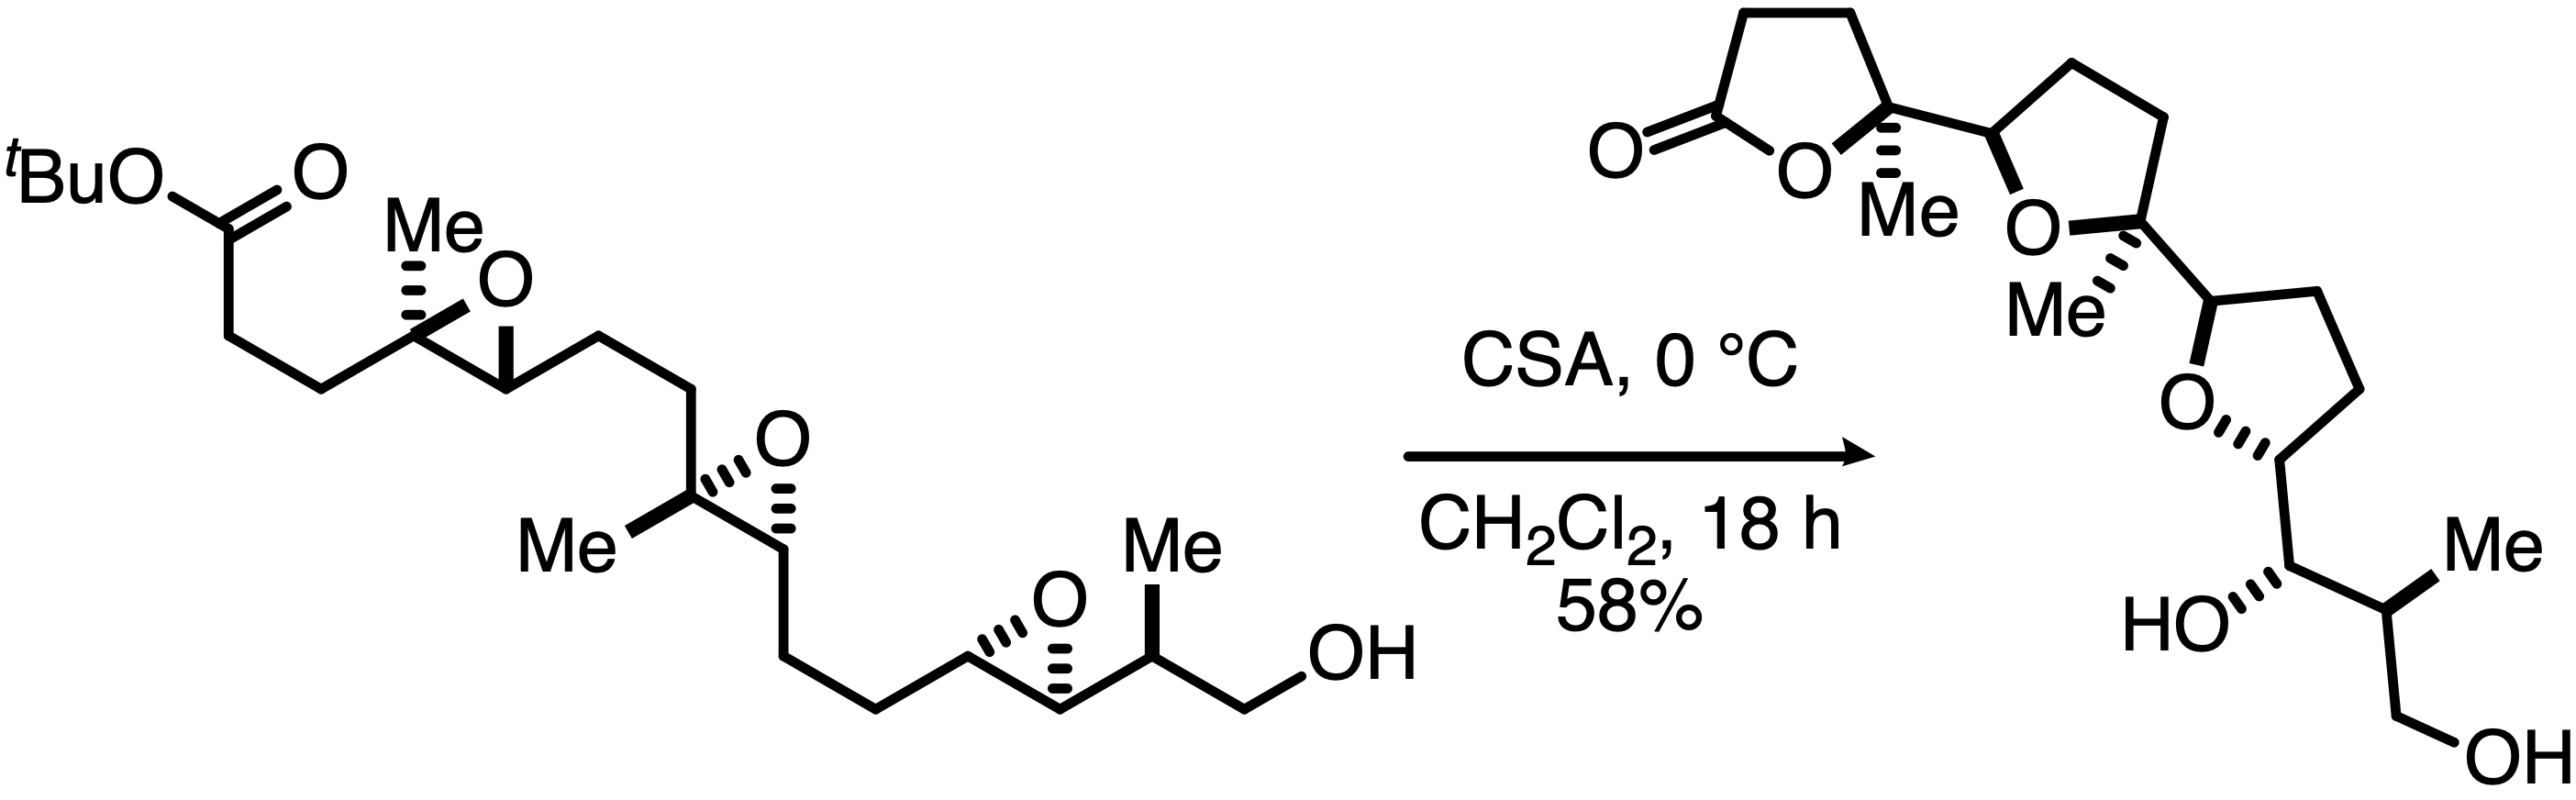
\includegraphics[width=0.6\linewidth]{PSet2Q1.png}
        \caption{PSet 2, Q1.}
        \label{fig:PSet2Q1}
    \end{figure}
    \item The distal epoxide carbons with methyl groups attached could hold stable carbocations, and thus be the beginning of an S\textsubscript{N}1 mechanism.
    \begin{itemize}
        \item Alternatively, the distal epoxide carbons without methyl groups attached are open to S\textsubscript{N}2 attacks.
    \end{itemize}
    \item There appears to be a stereoinversion at C3. Could this be due to attack by the conjugate base after activation?
    \begin{itemize}
        \item But then how would CSA snap off to leave behind an alcohol?
    \end{itemize}
    \item It probably would make the most sense to have the cascade go up the chain, terminating by kicking out \emph{t}-butoxide.
    \item How is the stereochemistry set?
    \begin{itemize}
        \item This is an example from Ian Patterson in the 1970s.
        \item Jasmin's overall strategy is correct.
        \item Acid-catalyzed loss of a \emph{t}-butyl group is correct! We have a \emph{t}-butyl cation that will either be trapped (solvation), or it will eliminate to regenerate the acid.
    \end{itemize}
    \item Epoxides aren't super reactive on their own; they will need to be protonated to react.
    \begin{itemize}
        \item We do indeed have an S\textsubscript{N}1 mechanism.
        \item The $\pKa$ of an epoxide is $-2$, but for CSA, it's 1.2!
        \item We can't easily do an S\textsubscript{N}2 on epoxides!
        \item Epoxides are unique under electrophilic conditions in that they can draw in a nucleophile (even to a sterically hindered site) because there is so much energy in releasing the ring strain.
        \item You get more bond elongation on the tertiary distal carbon.
        \item The first step is a 5-exo-tet cyclization; epoxides \emph{can} do this chemistry.
    \end{itemize}
    \item Stereochemistry is inverted at every step; this is consistent with a stereospecific process.
    \item We should protonate the oxygen of the carbonyl; better, like in the amide because it doesn't break conjugation.
    \item The \emph{t}-butyl ester can add in, which is even better because t-butyl stabilizes a positive charge. We'll always use the carbonyl lone pair as a nucleophile; we don't use a carboxylic acid as a nucleophile.
    \item Very rapid protonation of all epoxides (relative to the protonation of the carbonyl). Once the end one is protonated, we'll have intramolecular addition.
    \item Amides and ethers both have lone pairs that can't be used.
    \begin{itemize}
        \item The lone pairs on the oxygen are equivalent.
        \item We don't use the bottom resonance picture because even if the ether oxygen is resonance-delocalized in with $sp^2$ hybridization, that oxygen is positively charged, so there's no way we'll use it as a nucleophile.
    \end{itemize}
    \item Good thing to observe about the starting material: Every step is stereoinvertive.
    \item Altogether, the full solution to PSet 2, Q1 is on the next page.
    \begin{figure}[h!]
        \centering
        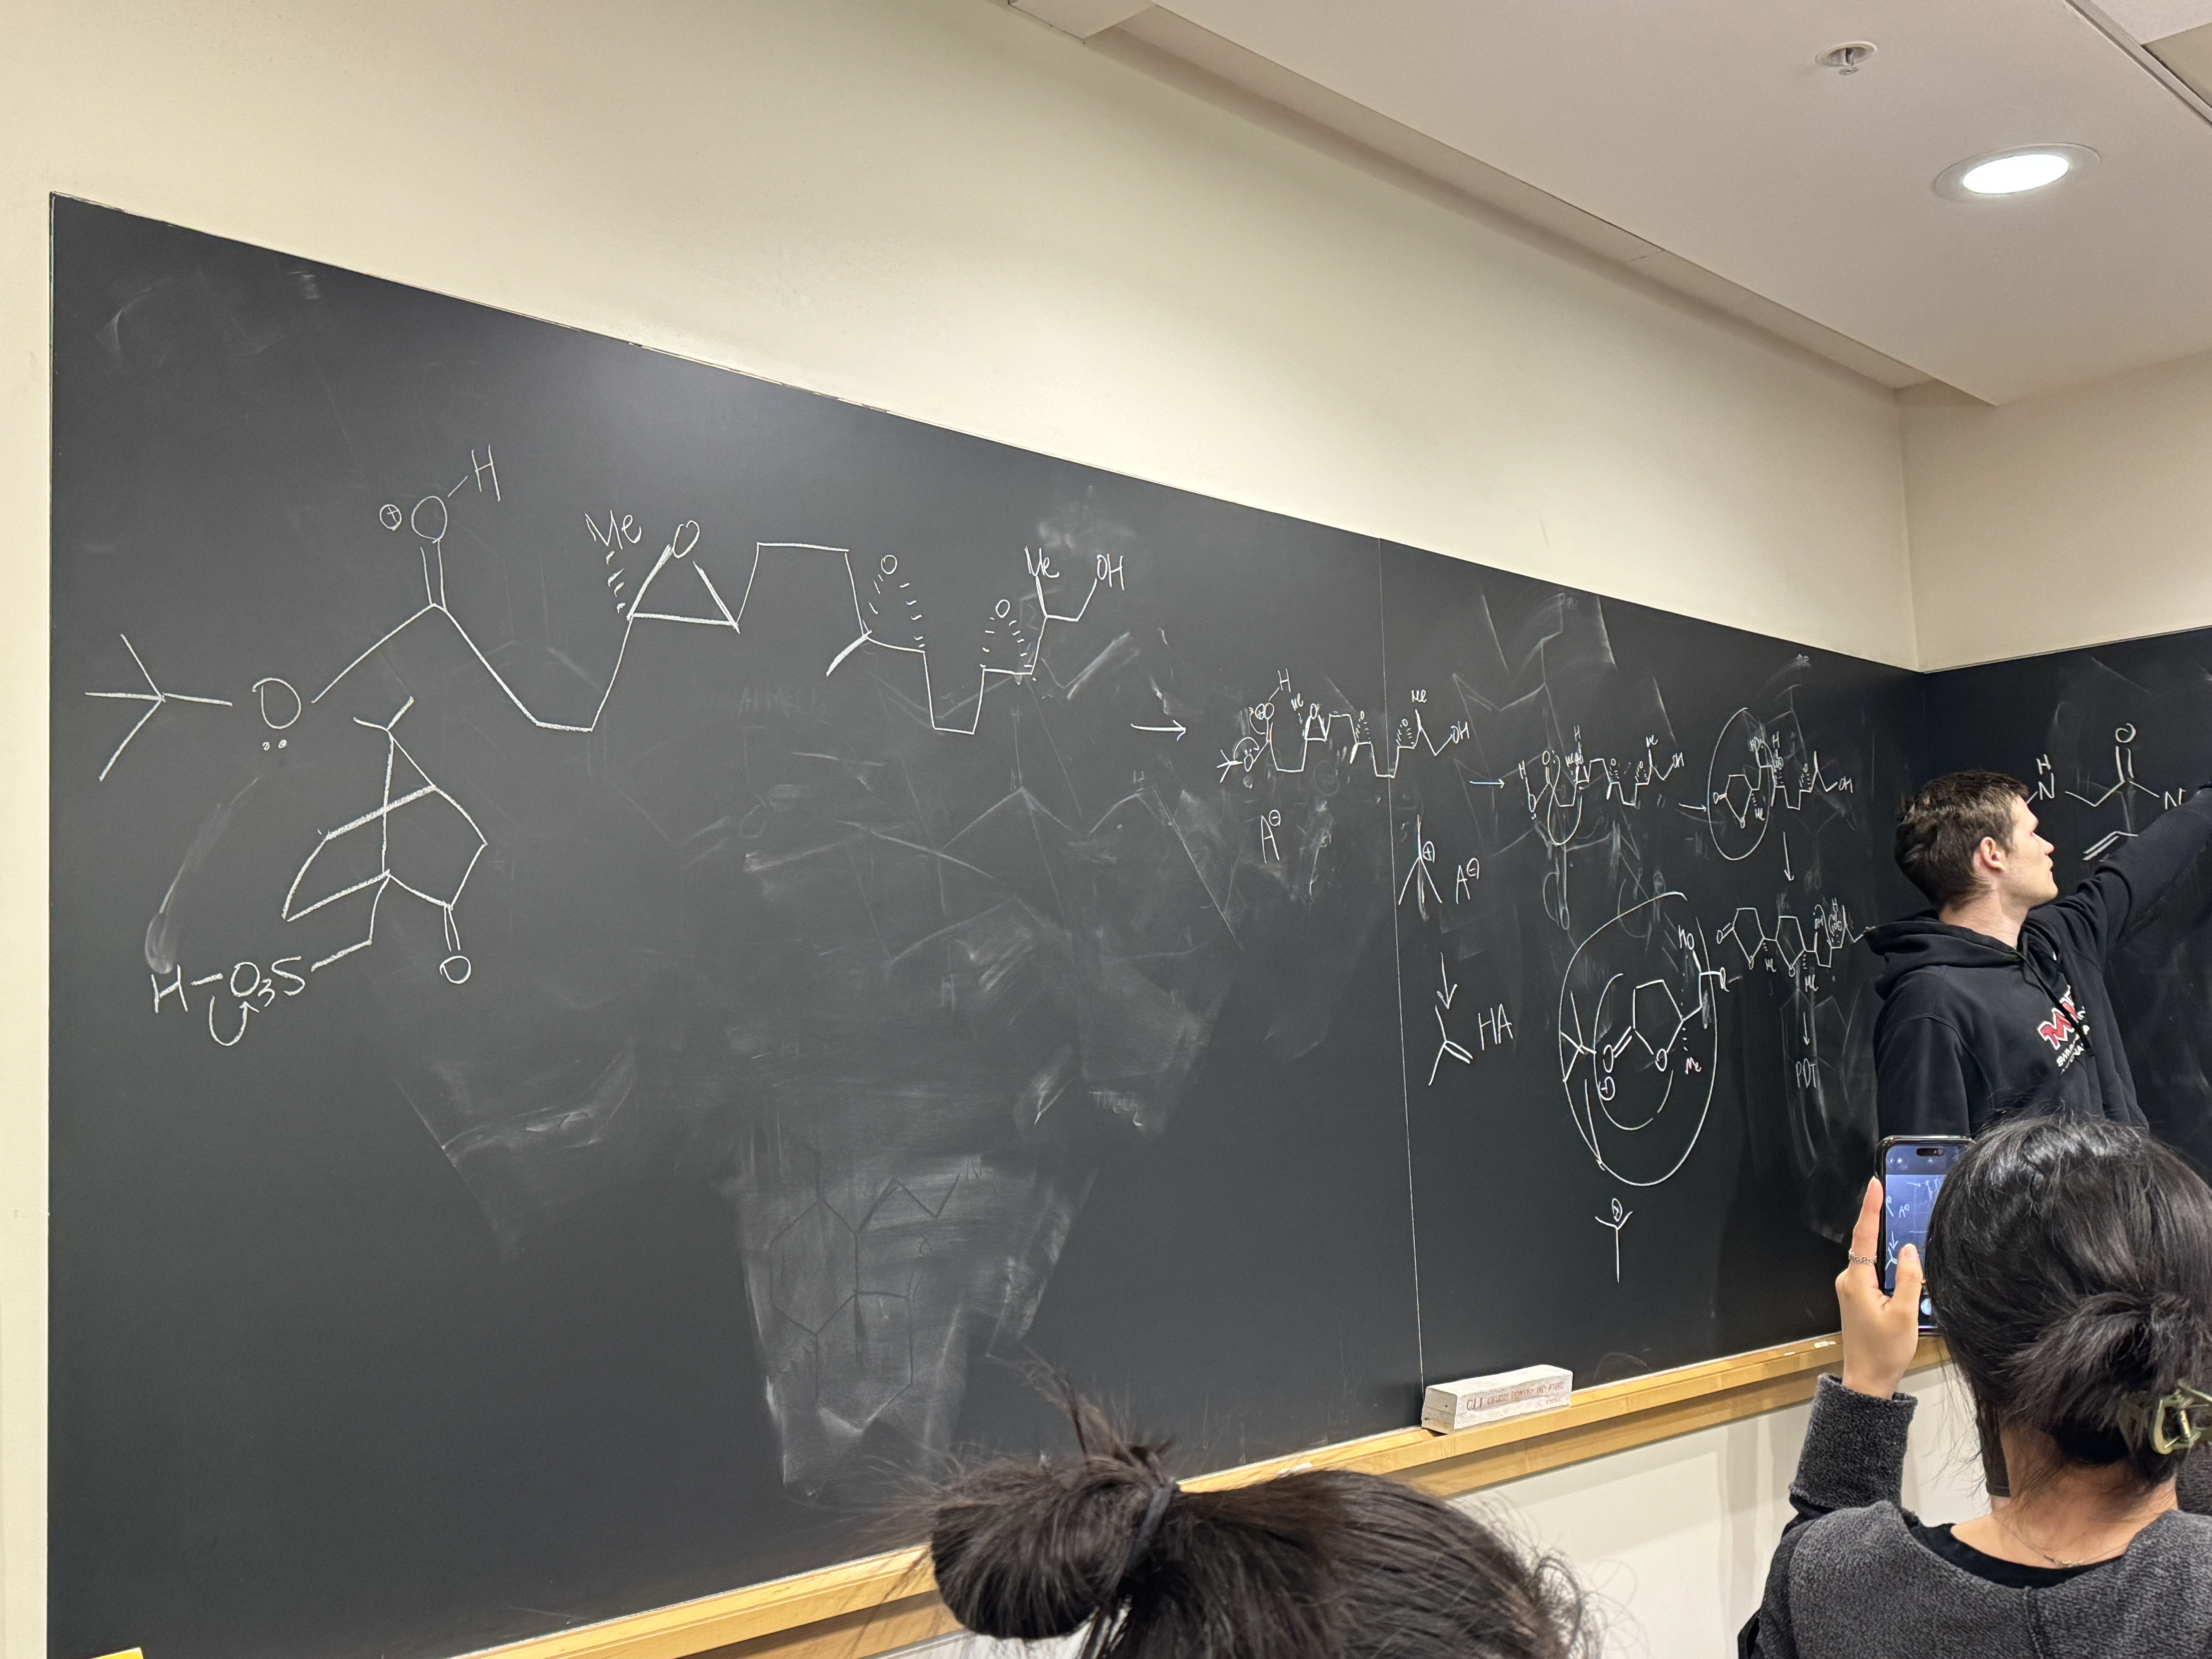
\includegraphics[width=0.8\linewidth]{PSet2Q1S.JPG}
        \caption{PSet 2, Q1 solution.}
        \label{fig:PSet2Q1S}
    \end{figure}
    \pagebreak
    \item We now begin discussing Problem 4.
    \begin{figure}[h!]
        \centering
        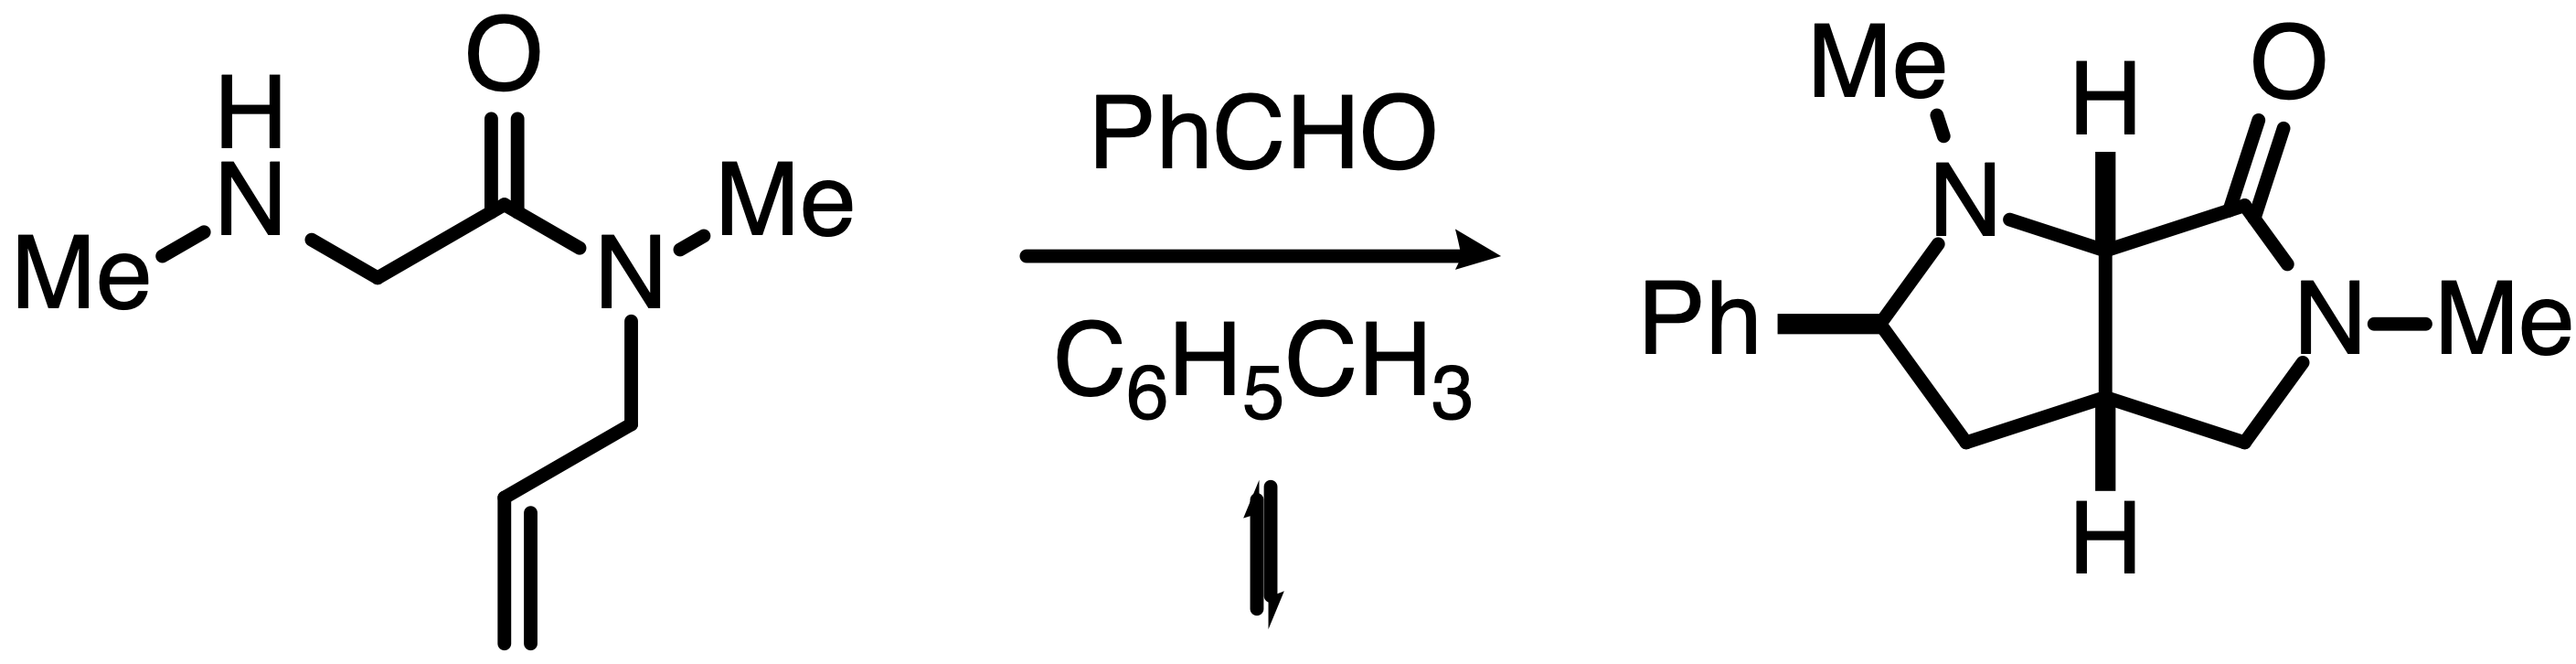
\includegraphics[width=0.45\linewidth]{PSet2Q4.png}
        \caption{PSet 2, Q4.}
        \label{fig:PSet2Q4}
    \end{figure}
    \item The heat is approximately \SI{110}{\celsius}.
    \item In \emph{some} order, we probably have aldehyde condensation to the iminium, a keto-enol tautomerization, and a $[3+2]$ cycloaddition.
    \item Stereochemistry gets set during the final cycloaddition analogous to the Diels-Alder.
    \begin{itemize}
        \item 5-5 ring system wants to be \emph{cis}-fused. And the phenyl will want to be on the outside.
    \end{itemize}
    \item The hydrogens are not too easy to enolize; the nitrogen pairs add electron density and make this $\pKa=25$ vs. $\pKa=20$ of acetone.
    \item We won't lose hydroxide and then use it; it will be intramolecular.
    \begin{itemize}
        \item 
    \end{itemize}
    \item This is a dipolar $[3+2]$ cycloaddition. You get a dipolarophile.
    \begin{itemize}
        \item You have true carbanion formation from deprotonation of the $\alpha$-hydrogen by the hydroxide in the hemiaminal intermediate; the hydroxide is our base.
        \item The $\alpha$-hydrogen will be labilized by both the iminium and the amide!
    \end{itemize}
    \item Altogether, the full solution to PSet 2, Q4 is on the next page.
    \begin{figure}[h!]
        \centering
        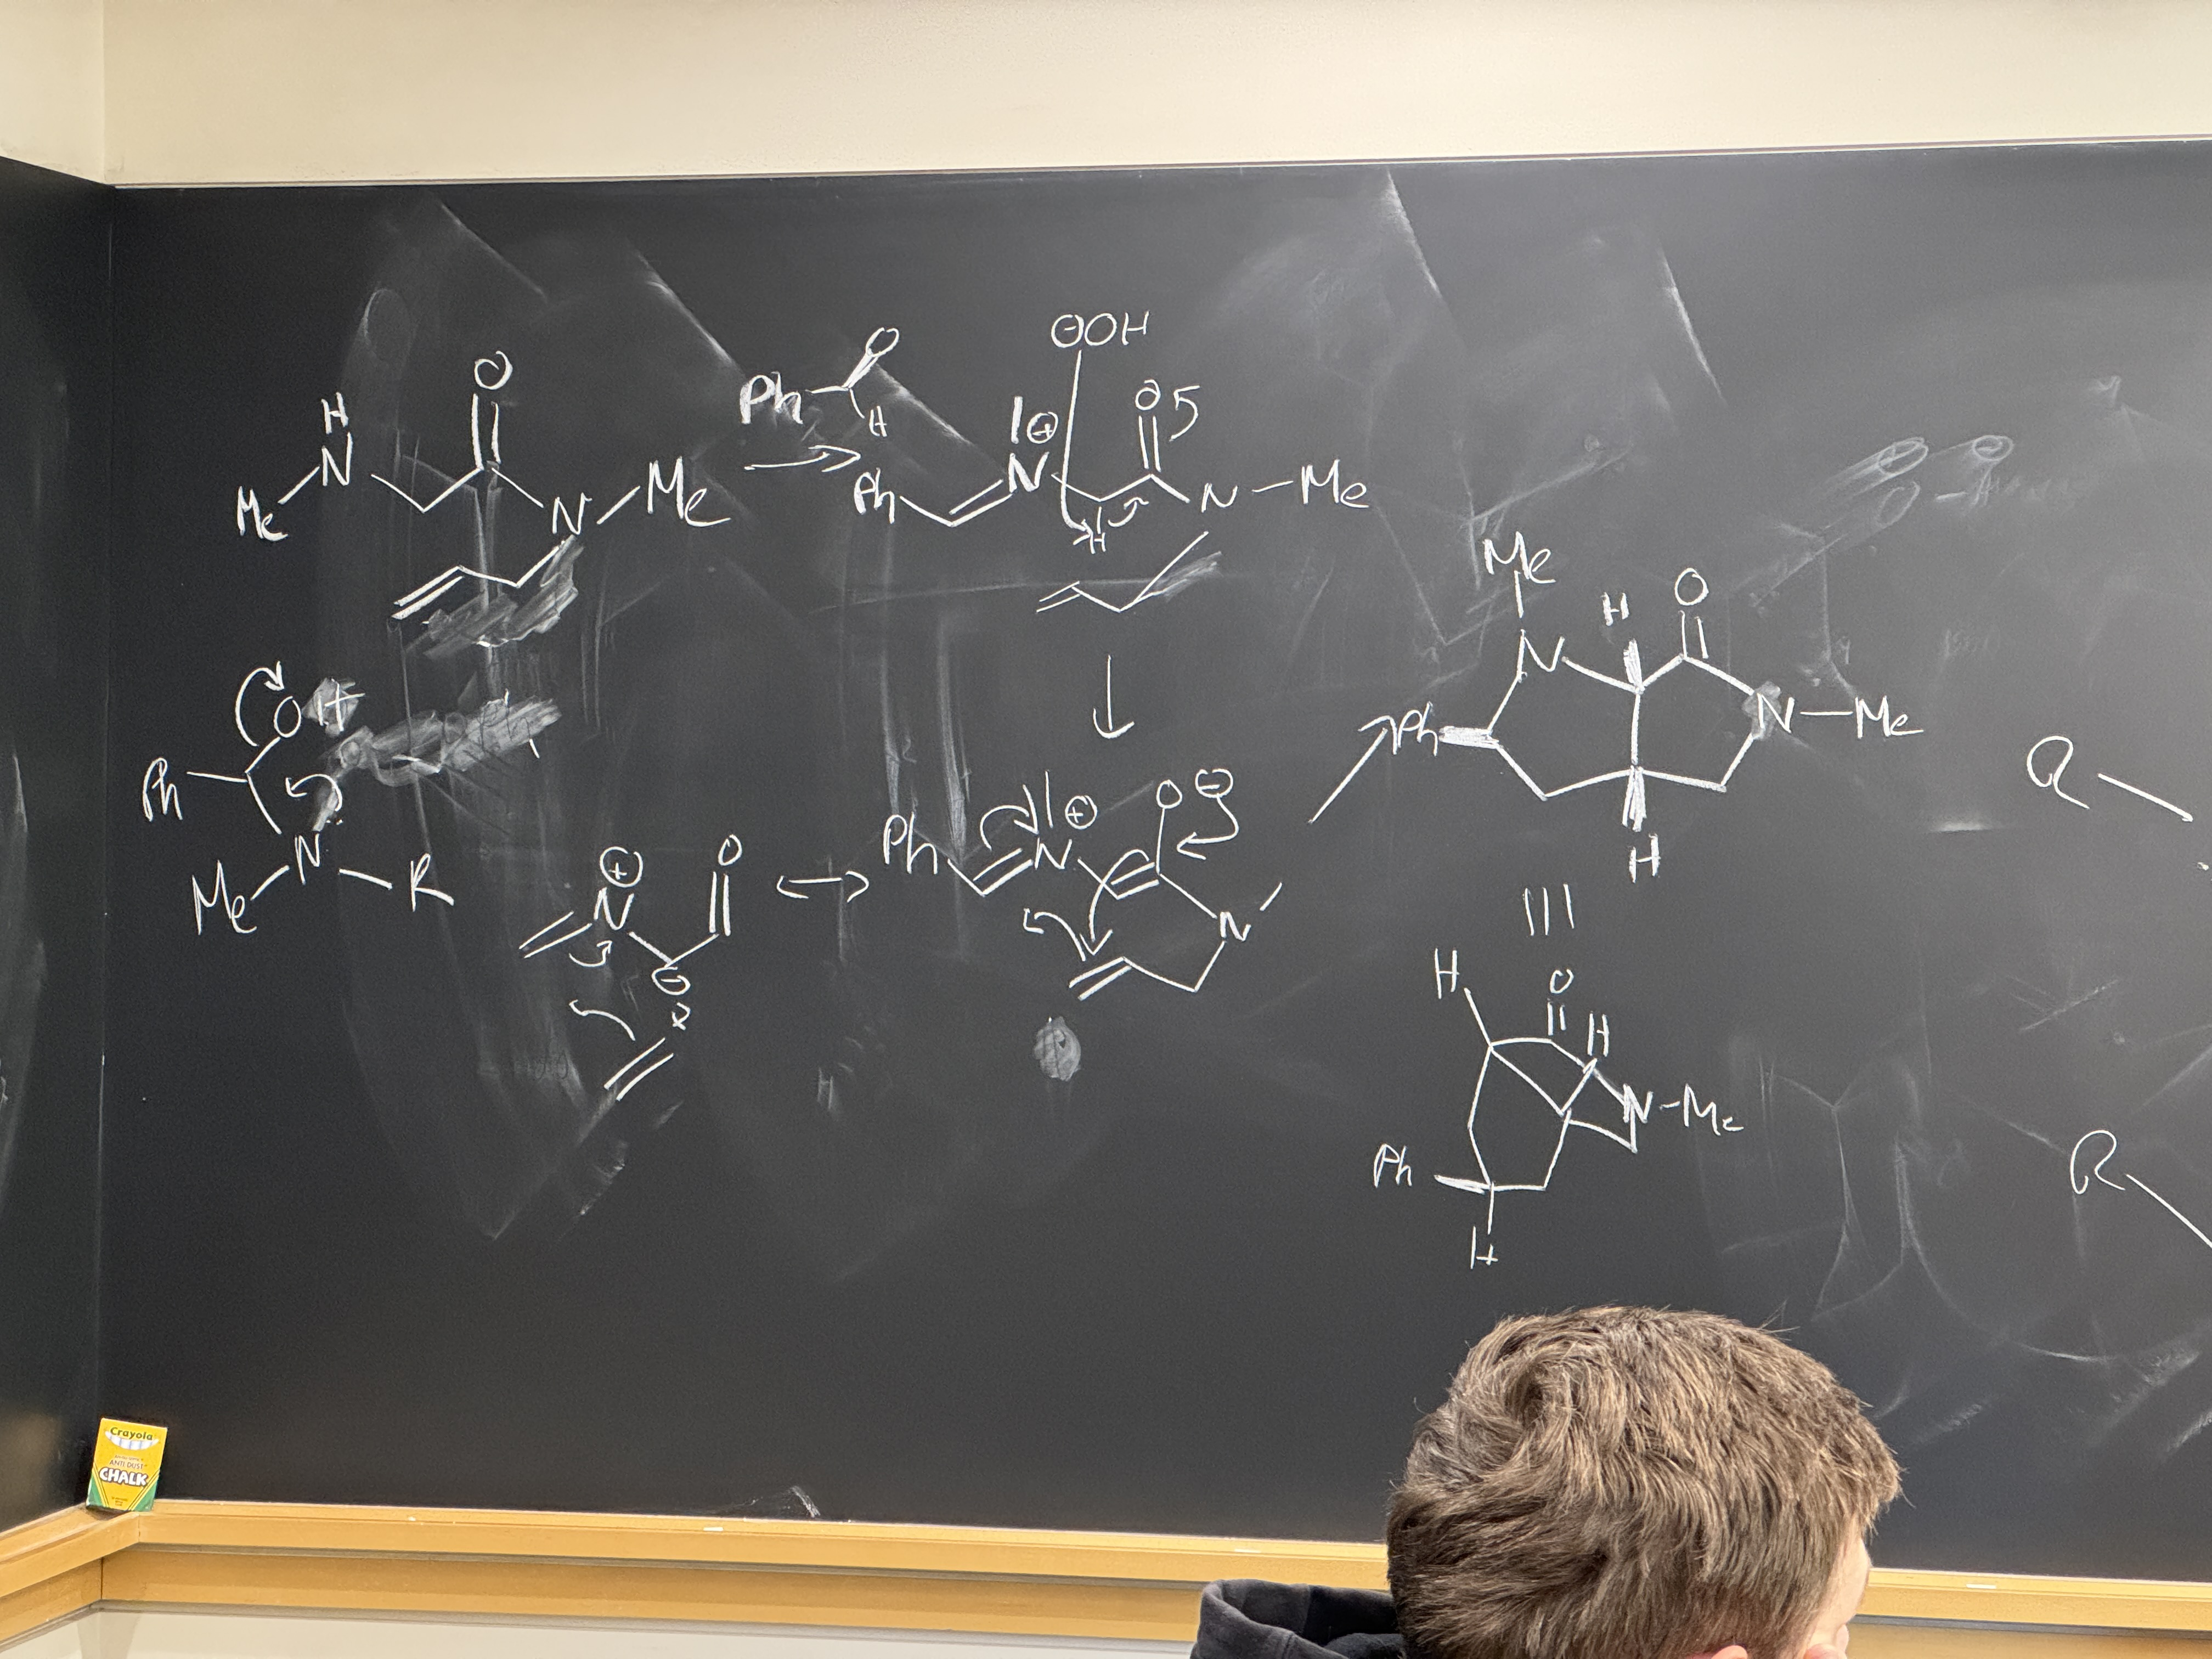
\includegraphics[width=0.7\linewidth]{PSet2Q4S.JPG}
        \caption{PSet 2, Q4 solution.}
        \label{fig:PSet2Q4S}
    \end{figure}
    \pagebreak
    \item We now begin discussing Problem 6 (Ivan).
    \begin{figure}[h!]
        \centering
        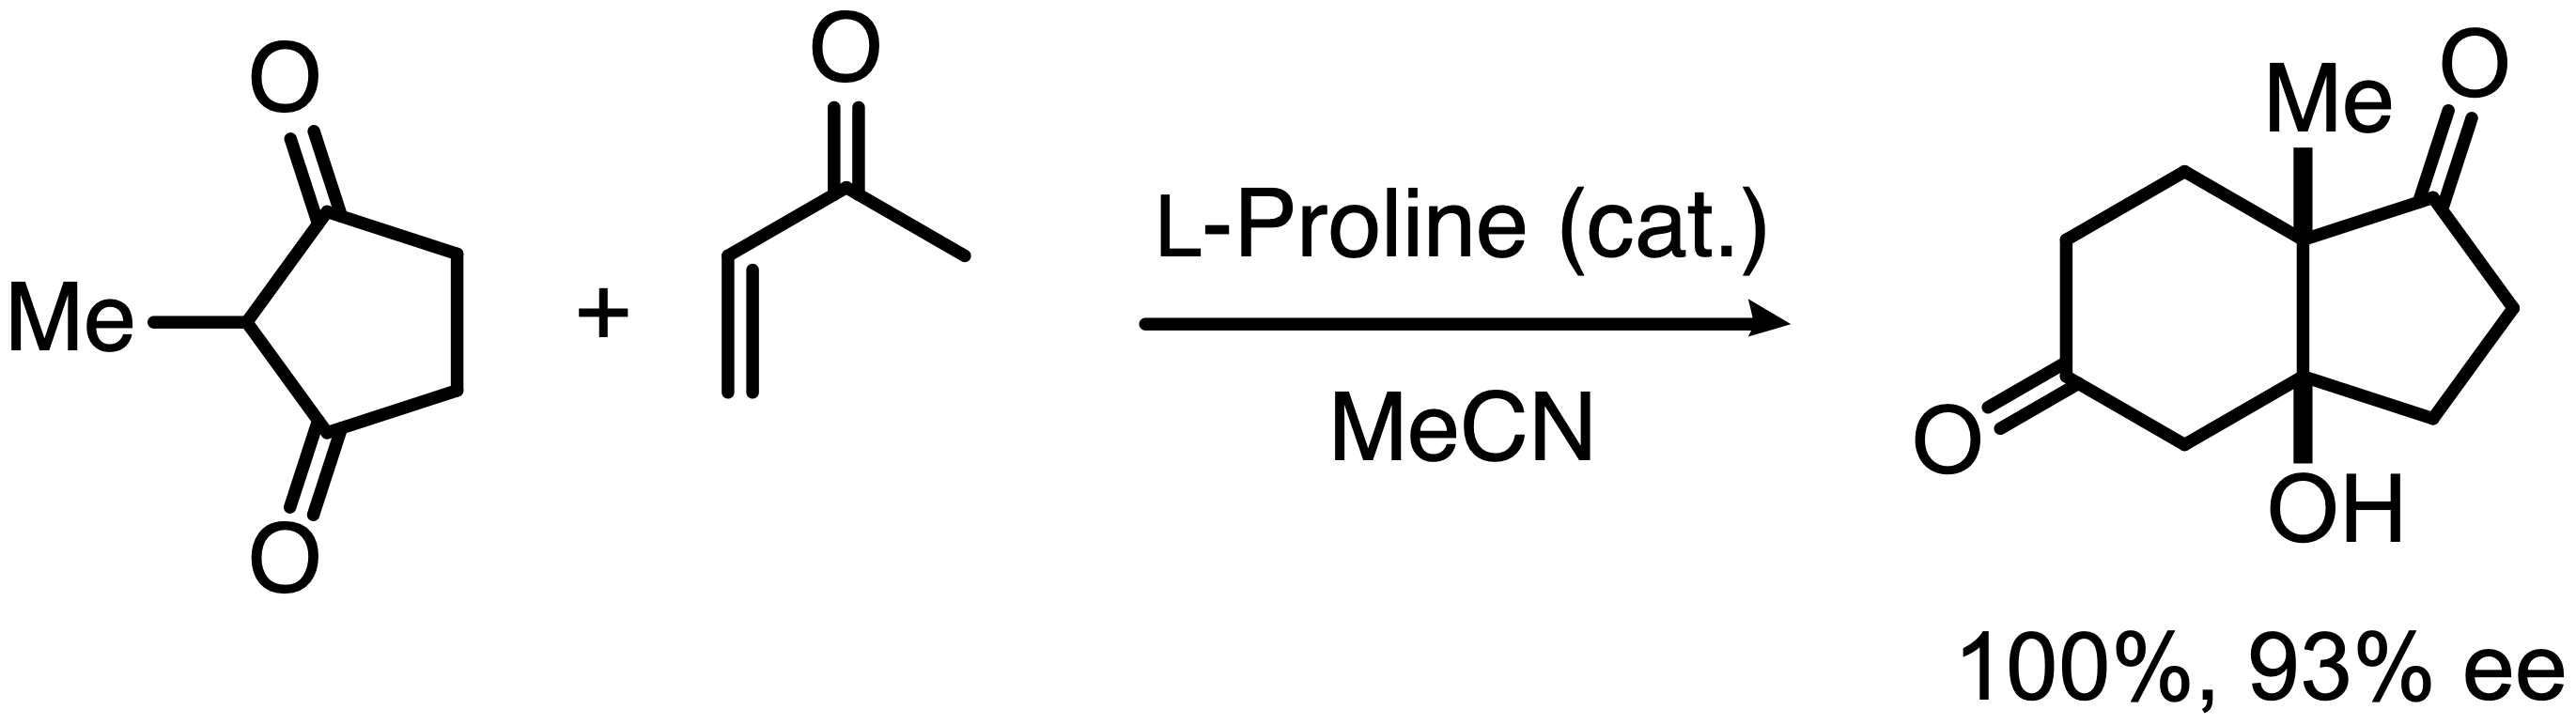
\includegraphics[width=0.45\linewidth]{PSet2Q6.png}
        \caption{PSet 2, Q6.}
        \label{fig:PSet2Q6}
    \end{figure}
    \item The core of this reaction is --- once again --- a cycloaddition. We get there by activating the $\alpha,\beta$-unsaturated ketone into a diene and the other species into a good dienophile. Then the chirality of the proline organocatalyst combined with the Diels-Alder diastereoselectivity gives us what we want.
    \item What provides the regioselectivity?? The diene does not have its EDG in an optimal position\dots
    \item The first step is conjugate addition, not condensation. You don't even need proline here before condensation. We do not form a stereocenter.
    \item The proline species in solution (by $\pKa$'s) is the carboxylate and the ammonium.
    \item Why the enamine targets the one ketone.
    \begin{itemize}
        \item It is more kinetically viable.
    \end{itemize}
    \item Altogether, the full solution to PSet 2, Q6 is on the next page.
    \begin{figure}[h!]
        \centering
        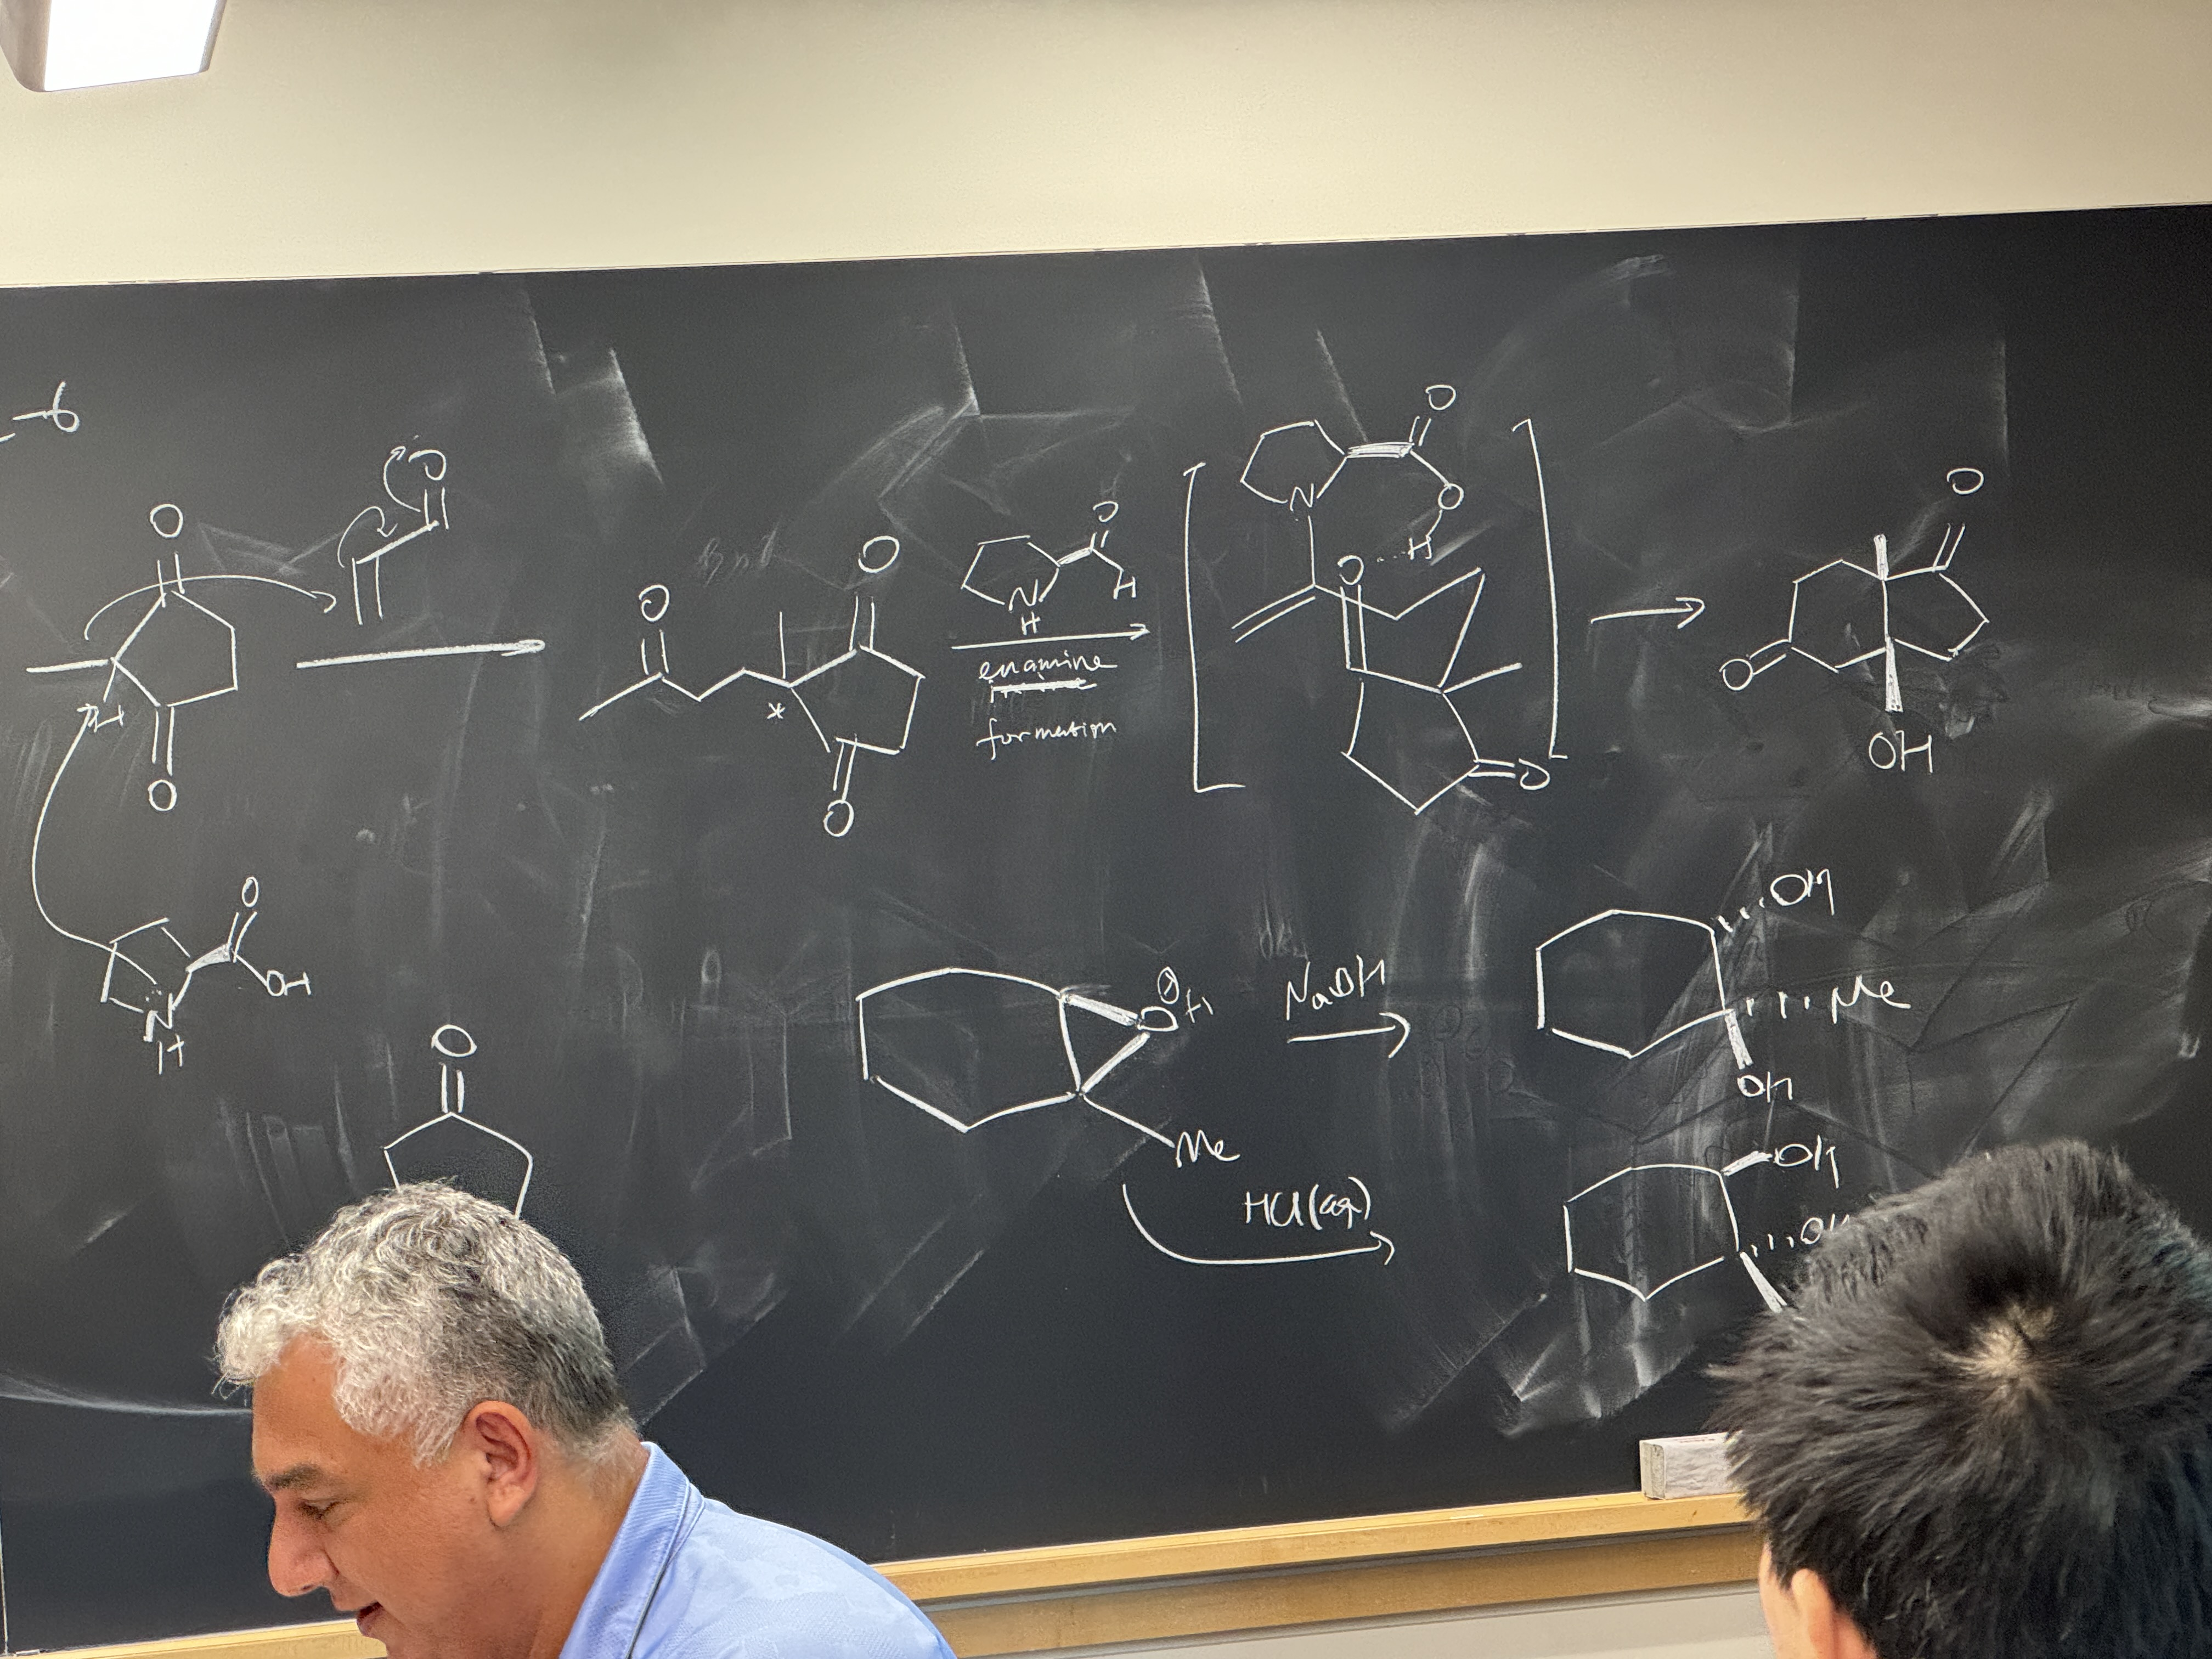
\includegraphics[width=0.8\linewidth]{PSet2Q6S.JPG}
        \caption{PSet 2, Q6 solution.}
        \label{fig:PSet2Q6S}
    \end{figure}
    \pagebreak
    \item Actually have a \emph{fully} worked out mechanism for any problem I'm supposed to present. Sketch it out \emph{and} try to fully work it out. Drawing it all out will end up saving time and catching mistakes!!
    \item He'll ask us at the beginning of next class which PSet 3 problems we found the most difficult/interesting.
    \item Jeremiah will be here on Wednesday; Mo will be back on Friday.
    \begin{itemize}
        \item Jeremiah will send us a PSet for Wednesday. Mo will pick up with PSet 3 on Friday.
    \end{itemize}
    \item Frank and Ivan started PSet 3; nobody else did.
    \begin{enumerate}
        \item Really good use of 3D transition states. Note the use of the semicolon; other reagents aren't present in the first step. Something happens with the acid, then with the diazo, then with the DMSO. Consider the Swern oxidation. Perchloric acid is useful for a reason.
        \item More of a carbocation pathway. Think about the coordination of the ??, ring strain release, no NaBh4 before the skeleton is formed. Last step is jsut reducation.
        \item Very interesting. Consider Friedel-Crafts type chemistry, and a symmetrical intermediate. This helps explain the product distrubiton/formaiton of product over SM. Protonation states are important here.
        \item Two consecutive photochemical steps. Aminal intermediate, H-atom abstraction chemistry.
        \item The ynolate (negatively charged oxygen center) is like an enolate; very nucleophilic, very sterically accessible. Notice the refluxing condition. Silica gel indicates protic conditions.
        \item Aldol chemistry.
    \end{enumerate}
\end{itemize}




\end{document}